% !TEX root = report.tex

\subsection{Correlation matrix}
\label{app:correlation_matrix}
In the large figure \ref{fig:correlation_matrix} is represented the correlation matrix among the 55 different high-level audio features (or, better, distributions) that have been extracted from each clip of ESC-50, according to the procedure explained in section \ref{sec:features_extraction}.\\
Analyzing this correlation matrix we can make several interesting observations about the information that has been effectively extracted from the audio samples:
\begin{itemize}
	\itemsep0em
	\item as expected, variables that are already "grouped", like MFCCs, chroma features, etc. manifest some kind of dependence among each other (especially the variables in the chromagram, that appear to be strongly correlated);
	\item spectral features and zero-crossing rate, even if computed separately, as "single" features, exhibit some correlations; the reason is that they simply all come from the analysis of the same spectrogram;
	\item spectral features and MFCCs seems somehow anti-correlated;
	\item energy and corresponding derivatives are less likely to reveal any kind of dependence with any other variable;
	\item an interesting correlation appears between the MFCCs and the chroma features;
	\item just to precise, many of the anti-correlations involving the deltas that can be evinced from the plot are originated simply by the fact that such features are directly calculated from the others and so the dependence is obvious.
\end{itemize}

So, to conclude, many of the features extracted exhibit some kind of correlations/anti-correlations among each other, and for this reason they probably share part of the information carried. Further proof of this conclusion can be found in appendix \ref{app:dim_reduction}, when talking about Principal Component Analysis.

\begin{figure*}[t]
	\centering
	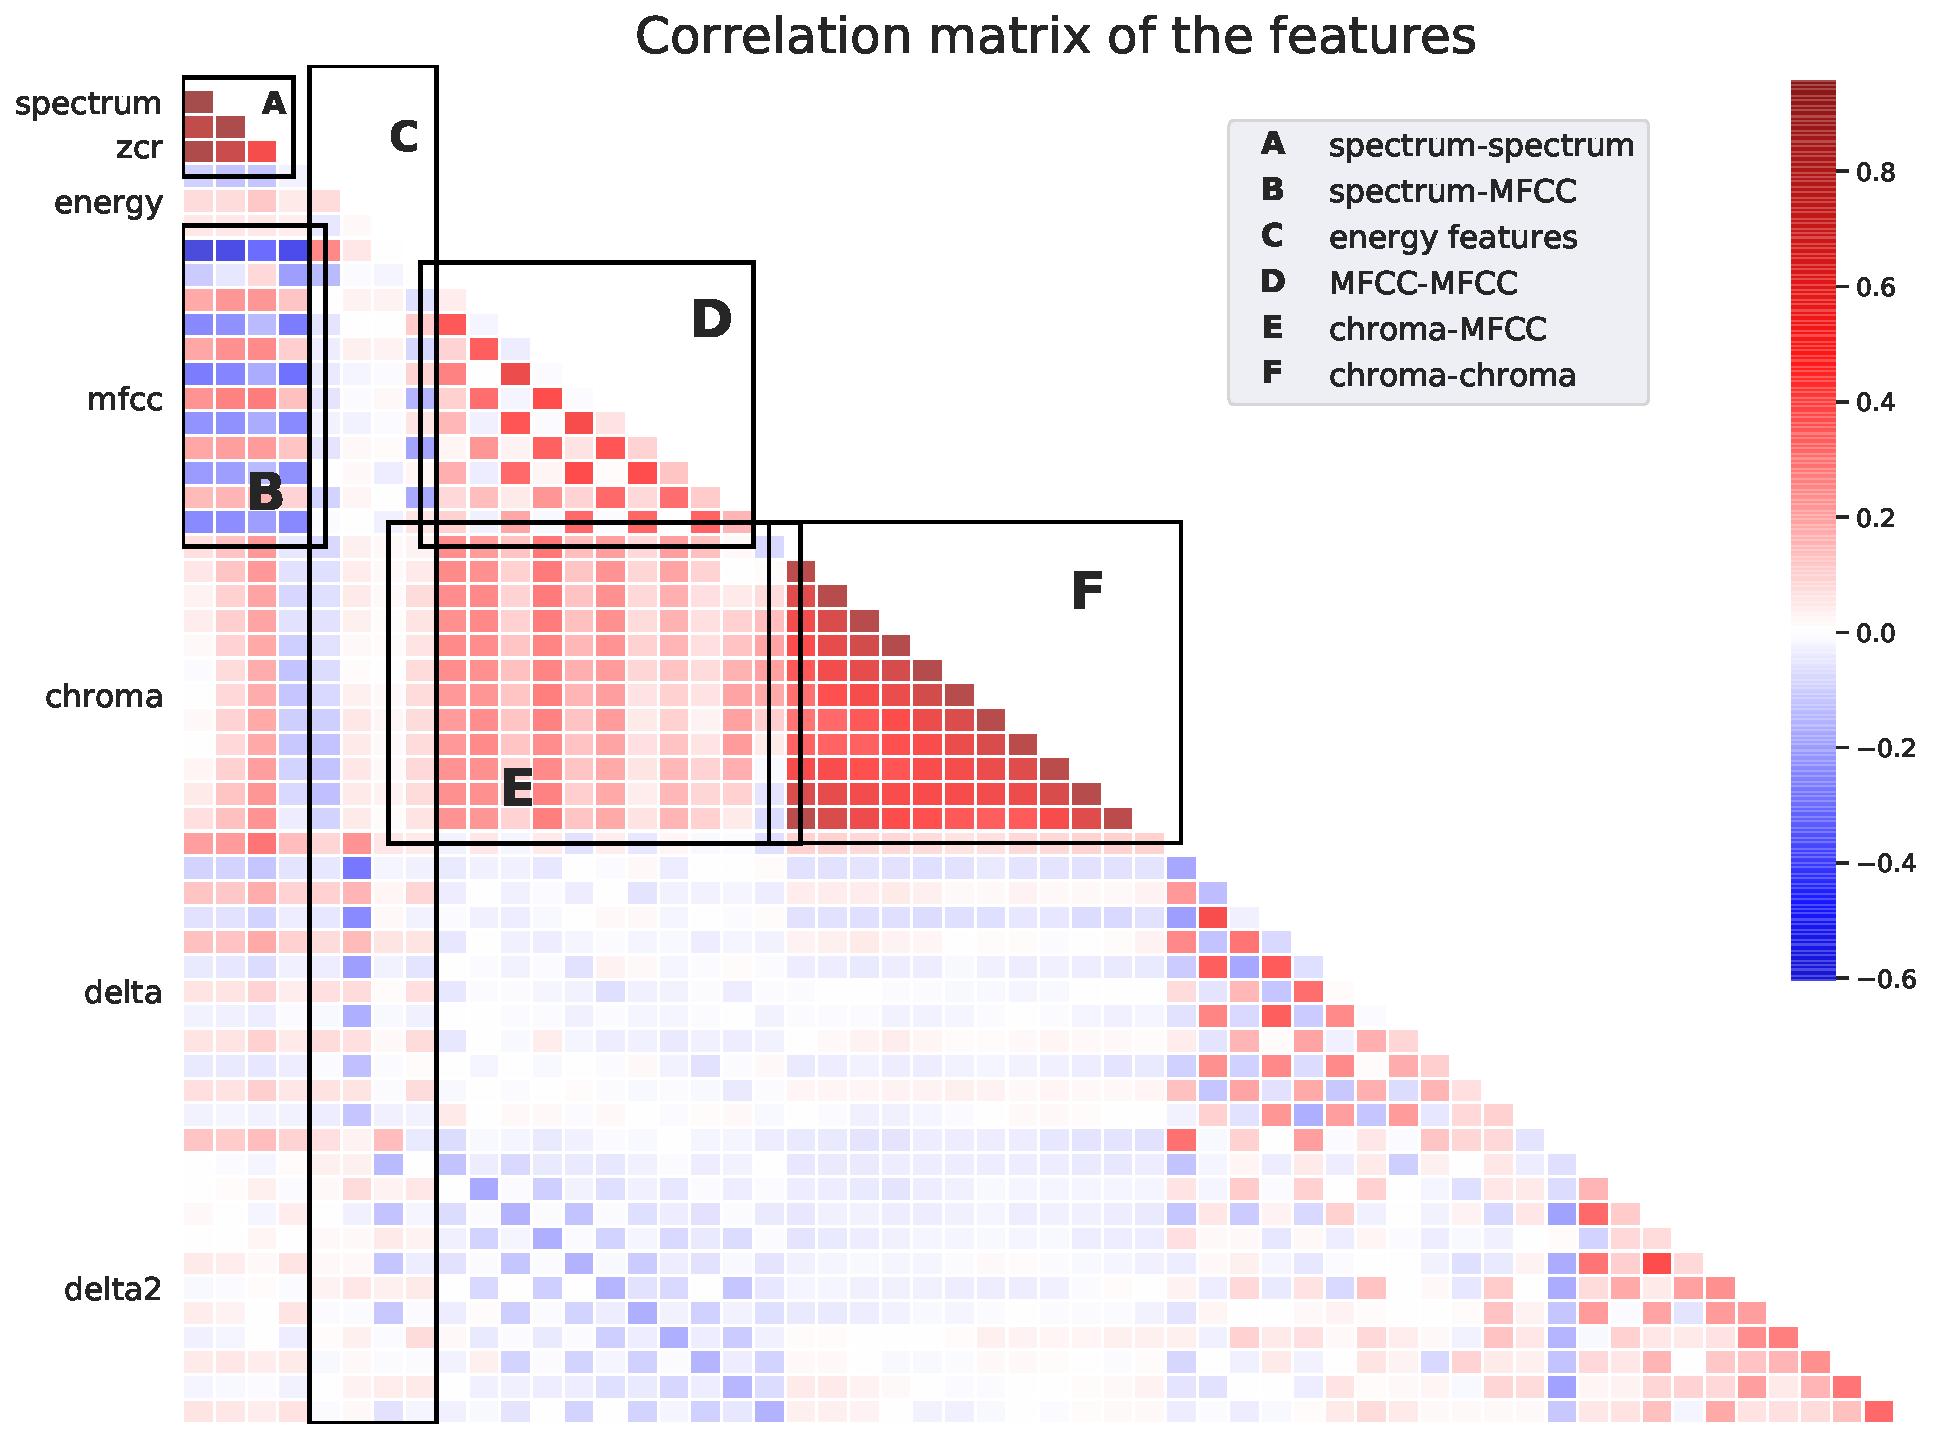
\includegraphics[scale=0.5]{pictures/correlation_matrix}
	\caption{Correlation matrix of the 55 high-level audio features extracted to represent the clips contained in ESC-50, as explained in section \ref{sec:features_extraction}.}
	\label{fig:correlation_matrix}
\end{figure*}